\documentclass[10pt,a4paper]{article}
\usepackage[utf8]{inputenc}
\usepackage[italian]{babel}
\usepackage{amsmath}
\usepackage{amsfonts}
\usepackage{float}
\usepackage{amssymb}
\usepackage{graphicx}
\graphicspath{ {./images/} }
\author{Gianluca Mondini}
\title{Tesi (titolo da definire)}
\begin{document}

\begin{center}
\textbf{Attenzione: il seguente documento è ancora in fase di stesura, pertanto presenta sezioni abbozzate, incorrette ed incomplete.}
\end{center}

\maketitle

%\pagebreak

%\tableofcontents

%\pagebreak

\section{Obiettivo}

Implementazione dell'algoritmo di Lloyd per l'equidistribuzione di uno sciame di droni su un'area specifica.

È prevista la realizzazione di un modulo che ...

\section{Il drone e sue componenti}

Possiamo schematizzare, ai fini di questa trattazione, un \textit{drone} mediante 3 componenti: il \textit{centro fisico}, il \textit{controllo di volo} e il \textit{controllo della traiettoria}\footnote{da rivedere i nomi dei 3 componenti}

\begin{center}
\textbf{Inserire qui uno schemino che illustri i tre componenti del drone}
\end{center}

\subsection{Centro fisico}

Il centro fisico è un astrazione che rappresenta il rapporto del drone con il mondo esterno. Vengono quindi qui considerati parametri la massa, la velocità, l'accelerazione, la posizione, la rotazione, la velocità di rotazione dei motori e la potenza che viene fornita a questi.

\section{Algoritmo di Lloyd}

\subsection{Introduzione}

L'algoritmo di Lloyd, conosciuto anche con il nome di \textit{iterazione di Voronoi}, è un algoritmo che permette di ...

\subsection{Descrizione}

L'algoritmo esegue ripetutamente i seguenti \textit{step}:

\begin{enumerate}
	\item Viene generato il diagramma di Voronoi
	\item Per ogni cella trovata, viene determinato il \textit{baricentro}
	\item Ogni punto viene spostato in corrispondenza del \textit{baricentro} della propria \textit{cella di Voronoi}
\end{enumerate}

\subsection{Esempio di applicazione dell'algoritmo}

Viene qui presentata l'applicazione dell'algoritmo di Lloyd ad un'area quadrata nella quale sono presenti 5 partizioni.

Le croci rappresentano i \textit{baricentri} delle varie partizioni.

\begin{figure}[H]
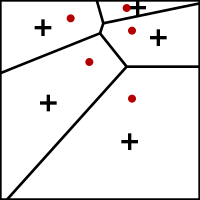
\includegraphics[width=5cm]{lloyd_iterazione_1.png}
\centering
\caption{I iterazione}
\end{figure}

\begin{figure}[H]
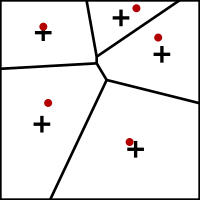
\includegraphics[width=5cm]{lloyd_iterazione_2.png}
\centering
\caption{II iterazione}
\end{figure}

\begin{figure}[H]
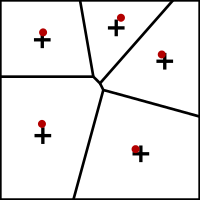
\includegraphics[width=5cm]{lloyd_iterazione_3.png}
\centering
\caption{III iterazione}
\end{figure}

\begin{figure}[H]
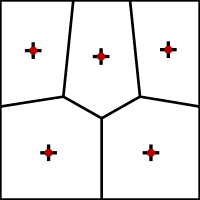
\includegraphics[width=5cm]{lloyd_iterazione_4.png}
\centering
\caption{IV iterazione}
\end{figure}

\subsection{Convergenza dell'algoritmo}

Intuitivamente, si può dire che l'algoritmo converga in quanto i punti che si trovano a minor distanza tra loro tendono a compiere un movimento più alto, mentre i punti che si trovano a distanze elevate tendono a muoversi meno.


\section*{Bibliografia}

\begin{itemize}
	\item https://en.wikipedia.org/wiki/Lloyd\%27s\_algorithm
\end{itemize}

\end{document}